%
% Homework Details
%   - Title
%   - Due date
%   - University
%   - Class
%   - Class Alias
%   - Class Section
%   - Instructor
%   - Author
%   - AuthorID
%

\newcommand{\hmwkID}{3}
\newcommand{\hmwkTitle}{Homework\ \#\hmwkID}
\newcommand{\hmwkDueDate}{April 28, 2015 at 16:20}
\newcommand{\hmwkUniversity}{NTU}
\newcommand{\hmwkClass}{Data Structures and Algorithms}
\newcommand{\hmwkClassAlias}{DSA}
\newcommand{\hmwkClassSection}{Spring 2015}
\newcommand{\hmwkClassInstructor}{Hsuan-Tien Lin, Roger Jang}
\newcommand{\hmwkAuthorName}{Tim Liou}
\newcommand{\hmwkAuthorID}{b03902028}


\documentclass[11pt]{article}

\usepackage{fancyhdr}
\usepackage{extramarks}
\usepackage{enumitem}
\usepackage{amsmath}
\usepackage{amsthm}
\usepackage{amsfonts}
\usepackage{tikz}
\usepackage[plain]{algorithm}
\usepackage{algpseudocode}
\usepackage{listings}
\usepackage{lastpage}
\usepackage{color}

\usetikzlibrary{shapes,positioning,arrows,calc}
\usetikzlibrary{automata,positioning}

%
% Basic Document Settings
%

\topmargin=-0.45in
\evensidemargin=0in
\oddsidemargin=0in
\textwidth=6.5in
\textheight=9.0in
\headsep=0.25in

\linespread{1.1}

\pagestyle{fancy}
\lhead{\hmwkAuthorName\ (\hmwkAuthorID)}
\chead{\hmwkClassAlias\ (\hmwkUniversity, \hmwkClassSection): \hmwkTitle}
\rhead{\firstxmark}
\lfoot{\lastxmark}
\cfoot{\thepage\ of \pageref{LastPage}}

\renewcommand\headrulewidth{0.4pt}
\renewcommand\footrulewidth{0.4pt}

\setlength\parindent{0pt}
\setlength{\parskip}{1em}
%
% Create Problem Sections
%

\newcommand{\enterProblemHeader}[1]{
    \nobreak\extramarks{}{Problem \hmwkID.\arabic{#1} continued on next page\ldots}\nobreak{}
    \nobreak\extramarks{Problem \hmwkID.\arabic{#1} (continued)}{Problem \hmwkID.\arabic{#1} continued on next page\ldots}\nobreak{}
}

\newcommand{\exitProblemHeader}[1]{
    \nobreak\extramarks{Problem \hmwkID.\arabic{#1} (continued)}{Problem \hmwkID.\arabic{#1} continued on next page\ldots}\nobreak{}
    \stepcounter{#1}
    \nobreak\extramarks{Problem \hmwkID.\arabic{#1}}{}\nobreak{}
}

\setcounter{secnumdepth}{0}
\newcounter{partCounter}
\newcounter{homeworkProblemCounter}
\setcounter{homeworkProblemCounter}{1}
\nobreak\extramarks{Problem \hmwkID.\arabic{homeworkProblemCounter}}{}\nobreak{}

%
% Homework Problem Environment
%
% This environment takes an optional argument. When given, it will adjust the
% problem counter. This is useful for when the problems given for your
% assignment aren't sequential. See the last 3 problems of this template for an
% example.
%
\newenvironment{homeworkProblem}[2][-1]{
    \ifnum#1>0
        \setcounter{homeworkProblemCounter}{#1}
    \fi
    \section{\hmwkID.\arabic{homeworkProblemCounter} \hspace{0.1in} #2}
    \setcounter{partCounter}{1}
    \enterProblemHeader{homeworkProblemCounter}
}{
    \exitProblemHeader{homeworkProblemCounter}
}

%
% Title Page
%

\title{
    \vspace{2in}
    \textmd{\textbf{\hmwkClass:\ \hmwkTitle}}\\
    \normalsize\vspace{0.1in}\small{Due\ on\ \hmwkDueDate}\\
    \vspace{0.1in}\large{\textit{Instructors \hmwkClassInstructor}}
    \vspace{3in}
}

\author{
    \textbf{\hmwkAuthorName} \small{(\hmwkAuthorID)} 
}
\date{}

\renewcommand{\part}[1]{\textbf{\large Part \Alph{partCounter}}\stepcounter{partCounter}\\}

\lstset{
    language=C,
    numbers=left,
    frame=single,
    columns=fullflexible,
    basicstyle=\ttfamily
}

%
% Various Helper Commands
%

\newcommand{\subqest}[1]{ \textbf{(\arabic{partCounter})} #1 \stepcounter{partCounter} \par }

% Something need to be done
\newcommand{\pending}[1][]{~~~~\textcolor{red}{ 
        \textbf{ \large ====== Pending 
            \ifx&#1&%
            % #1 is empty
            \else
            % #1 is nonempty
            \large (#1)
            \fi
            \large ====== 
        } 
    }
}

% Useful for algorithms
\newcommand{\alg}[1]{\textsc{\bfseries \footnotesize #1}}

% For derivatives
\newcommand{\deriv}[1]{\frac{\mathrm{d}}{\mathrm{d}x} (#1)}

% For partial derivatives
\newcommand{\pderiv}[2]{\frac{\partial}{\partial #1} (#2)}

% Integral dx
\newcommand{\dx}{\mathrm{d}x}

% Alias for the Solution section header
\newcommand{\solution}{\textbf{\large Solution}}

% Probability commands: Expectation, Variance, Covariance, Bias
\newcommand{\E}{\mathrm{E}}
\newcommand{\Var}{\mathrm{Var}}
\newcommand{\Cov}{\mathrm{Cov}}
\newcommand{\Bias}{\mathrm{Bias}}




\begin{document}

\pagenumbering{gobble}

\maketitle

\pagebreak

\pagenumbering{arabic}  

\begin{homeworkProblem}{Asymptotic Complexity}
    \subqest{Do Exercise R-4.28 of the textbook.}
    Consider $a_k \geq 0~for~k \geq 0$
    \[
        \begin{split}
            p(n) = a_0 + a_1n + a_2n^2 + a_3n^3 + \dots + a_mn^m
        \end{split}
    \]

    For $n \geq (a_0 + a_1 + a_2 + \dots + a_m) \geq 1$, we have
    \[
        \begin{split}
            p(n) &\leq (a_0 + a_1 + a_2 + \dots + a_m) \times n^m
            \\
            \Rightarrow \log p(n) &\leq \log (a_0 + a_1 + a_2 + \dots + a_m) + m\log n
            \\
            &\leq \log n + m \log n
            \\
            &= (m+1) \log n
        \end{split}
    \]
    Take $c = m+1 > 0$, $n_0 = (a_0 + a_1 + a_2 + \dots + a_m) \geq 1$
    \[
        \begin{split}
            \log p(n) \leq c\log n~~for~n \geq n_0
        \end{split}
    \]
    That is, $\log p(n)$ is $O(\log n)$.


    \subqest{Do Exercise R-4.34 of the textbook.}
    We have $f(n) > 1$ and $\lceil f(n) \rceil \leq f(n) + 1$ by definition. For $n \geq 1$,
    \[
        \begin{split}
            \lceil f(n) \rceil &\leq f(n) + 1
            \\
            &\leq f(n) + f(n)
            \\
            &= 2f(n)
        \end{split}
    \]
    Take $c = 2 > 0$, $n_0 = 1 \geq 1$
    \[
        \begin{split}
            \lceil f(n) \rceil \leq cf(n)~~for~n \geq n_0
        \end{split}
    \]
    That is, $\lceil f(n) \rceil$ is $O(f(n))$.


    \subqest{Prove that $f(n) = \Theta(g(n))$.}
    By definition of limits at infinity,
    \[
        \begin{split}
            \lim_{n \to \infty} \frac{f(n)}{g(n)} = A
        \end{split}
    \]
    means that for every $\epsilon > 0$ there is a corresponding $N$ such that
    \[
        \begin{split}
            |\frac{f(n)}{g(n)} - A| < \epsilon ~~~for~n>N
        \end{split}
    \]

    That is,
    \[
        \begin{split}
            A - \epsilon < \frac{f(n)}{g(n)} < A + \epsilon ~~~for~n>N
        \end{split}
    \]

    Note that $g(n)$ is a strictly positive function. We have
    \[
        \begin{split}
            (A - \epsilon)g(n) < f(n) < (A + \epsilon)g(n) ~~~for~n>N
        \end{split}
    \]

    Take $\epsilon \in (0,A)$, $c_1 = (A - \epsilon) > 0$, $c_2 = (A + \epsilon) > 0$, $n_0 > N$
    \[
        \begin{split}
            c_1 g(n) \leq f(n) \leq c_2 g(n) ~~~for~n>n_0
        \end{split}
    \]
    This shows that $f(n) = \Theta(g(n))$.


    \subqest{Do Exercise R-4.8 of the textbook.}
    If A is better than B for $n \geq n_0$, $n_0$ satisfies the following statement.
    \[
        \begin{split}
            2{n_0}^3 - 40{n_0}^2 > 0
        \end{split}
    \]
    We can easily find that $n_0 > 20$. We choose $n_0 = 21$. It is a possible value for $n_0$ 
    satisfying the statement that A is better than B for $n \geq n_0$.
    
    
    \subqest{Do Exercise C-4.16(b) of the textbook.}
    This is the pseudo code of the Horner's method.
    \begin{algorithm}[]
        \begin{algorithmic}[1]
            \Function{Horner's-Method}{\emph{x,~CoefficientsOfPolynomial,~DegreeOfPolynomial}}
            \State{$Sum \gets 0$}
            \ForAll{\emph{CoefficientsOfPolynomial}}
                \State{$Sum \gets Sum \times x + \emph{CoefficientsOfPolynomial}$}
            \EndFor
            \State{\Return{$Sum$}}
            \EndFunction{}
        \end{algorithmic}
        \caption{Horner's method for computing polynomial}
    \end{algorithm}

    We can find there is only one \alg{for loop} in this pseudo code, that is, the number of 
    arithmetic operations is $O(n)$.


    \pagebreak

    \subqest{Consider some $f(n)$ and $g(n)$ such that $\lg f(n) = O(\lg g(n))$ and $g(n) \geq 2$
    for $n \geq 1$. Construct a counter-example to disprove that $f(n) = O(g(n))$.}
    Consider $f(n) = 4^n$, $g(n) = 2^n$, for $n \geq 1$, we can find
    \[
        \begin{split}
            \lg f(n) &= n 2 \lg 2 
            \\
            &\leq n 4\lg 2 
            \\
            &= 4 \lg 2^n
            \\
            &= 4\lg g(n)
        \end{split}
    \]

    Take $c = 4 > 0$, $n_0 = 1 \geq 1$
    \[
        \begin{split}
            \lg f(n) \leq c \lg g(n)~~for~n \geq n_0
        \end{split}
    \]
    That is, $\lg f(n)$ is $O(\lg g(n))$. Note that $g(n) \geq 2$ for $n \geq 1$.

    If $f(n) = O(g(n))$, $\exists n_0 > 0, c > 0 \ni$
    \[
        \begin{split}
            4^n \leq c 2^n~~for~n \geq n_0
        \end{split}
    \]
    Take $\log_2$ on both sides,
    \[
        \begin{split}
            &2n \leq \log_2 c + n~~for~n \geq n_0 \\
            &\Rightarrow n \leq \log_2 c 
        \end{split}
    \]
    Take $n^{\prime} = max(n_0, \lceil \log_2 c + 1 \rceil)$
    \[
        \begin{split}
            n^{\prime} \geq n_0 &\Rightarrow 4^n \leq c 2^n \\
            n^{\prime} > \log_2 c &\Rightarrow 4^n > c 2^n \\
        \end{split}
    \]
    This is a contradiction. Therefore, we disprove that $f(n) = O(g(n))$.

\end{homeworkProblem}

\pagebreak

\begin{homeworkProblem}{Stack, Queue, Deque}

    \subqest{Do Exercise C-5.2 of the textbook.}
    Pop out the elements in the stack one by one and check if it is equal to element $x$. After that,
    enqueue the elements into the queue one by one. Use a varible to store the number of the 
    elements we poped from the stack. Once we find the certain element or the stack is empty, we push
    the elements into stack from queue, and then enqueue the same number of element into queue from
    stack. Finally push all these elements from queue into stack again. This will maintain elements'
    original order.

    \begin{figure}[h!]
        \centering
        \begin{tikzpicture}[stack/.style={
                rectangle split, rectangle split parts=9, draw, anchor=center},
            myarrow/.style={single arrow, draw=none}]

            \node [stack] (s0)  {
            \nodepart{three}$e_n$\nodepart{four}$\vdots$\nodepart{five}$x$
            \nodepart{six}$\vdots$\nodepart{seven}$e_2$\nodepart{eight}$e_1$
            \nodepart{nine}$e_0$};
            \node [stack,right=of s0] (q0) {\nodepart{five}$\vdots$};
            \node [above=of s0,anchor=north,align=left] {S};
            \node [above=of q0,anchor=north,align=left] {Q};

            \node [myarrow,draw,right=of q0] (a1) {\phantom{te}} ;

            \node [stack,right=of a1] (s1)  {
            \nodepart{six}$\vdots$\nodepart{seven}$e_2$\nodepart{eight}$e_1$
            \nodepart{nine}$e_0$};
            \node [stack,right=of s1] (q1) {
            \nodepart{five}$x$
            \nodepart{six}$\vdots$\nodepart{seven}$e_{n-2}$\nodepart{eight}$e_{n-1}$
            \nodepart{nine}$e_n$};
            \node [above=of s1,anchor=north,align=left] {S};
            \node [above=of q1,anchor=north,align=left] {Q};

            \node [myarrow,draw,right=of q1] (a2) {\phantom{te}} ;

            \node [stack,right=of a2] (s2)  {
            \nodepart{three}$x$\nodepart{four}$\vdots$\nodepart{five}$e_n$
            \nodepart{six}$\vdots$\nodepart{seven}$e_2$\nodepart{eight}$e_1$
            \nodepart{nine}$e_0$};
            \node [stack,right=of s2] (q2) {\nodepart{five}$\vdots$};
            \node [above=of s2,anchor=north,align=left] {S};
            \node [above=of q2,anchor=north,align=left] {Q};

            \node [myarrow,draw,anchor=north] (a3) at ($(a1.south)+(0,-190pt)$) {\phantom{te}} ;

            \node [stack,right=of a3] (s3)  {
            \nodepart{six}$\vdots$\nodepart{seven}$e_2$\nodepart{eight}$e_1$
            \nodepart{nine}$e_0$};
            \node [stack,right=of s3] (q3) {
            \nodepart{nine}$x$
            \nodepart{eight}$\vdots$\nodepart{seven}$e_{n-2}$\nodepart{six}$e_{n-1}$
            \nodepart{five}$e_n$};
            \node [above=of s3,anchor=north,align=left] {S};
            \node [above=of q3,anchor=north,align=left] {Q};

            \node [myarrow,draw,right=of q3] (a4) {\phantom{te}} ;

            \node [stack,right=of a4] (s4)  {
            \nodepart{three}$e_n$\nodepart{four}$\vdots$\nodepart{five}$x$
            \nodepart{six}$\vdots$\nodepart{seven}$e_2$\nodepart{eight}$e_1$
            \nodepart{nine}$e_0$};
            \node [stack,right=of s4] (q4) {\nodepart{five}$\vdots$};
            \node [above=of s4,anchor=north,align=left] {S};
            \node [above=of q4,anchor=north,align=left] {Q};
        \end{tikzpicture}
        \caption{How this algorithm works}
    \end{figure}


    \pagebreak

    \subqest{Do Exercise C-5.9 of the textbook.}
    \begin{figure}[h!]
        \centering
        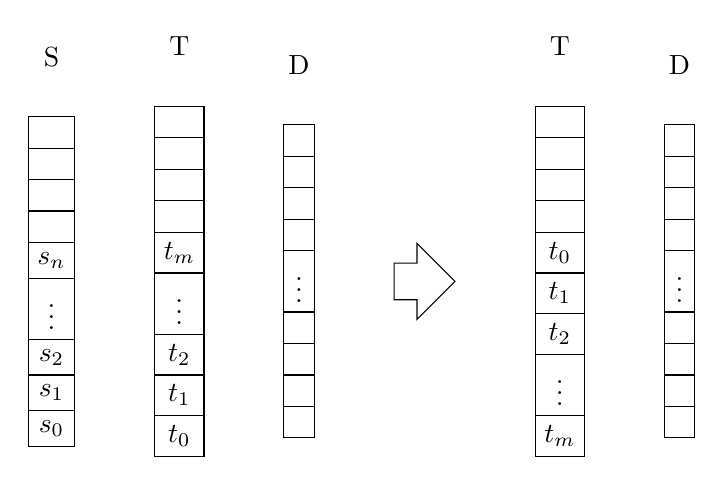
\begin{tikzpicture}[stack/.style={
                rectangle split, rectangle split parts=9, draw, anchor=center},
            myarrow/.style={single arrow, draw=none}]

            \node [stack] (s0)  {
            \nodepart{five}$s_n$
            \nodepart{six}$\vdots$\nodepart{seven}$s_2$\nodepart{eight}$s_1$
            \nodepart{nine}$s_0$};
            \node [stack,right=of s0] (t0) {
            \nodepart{five}$t_m$
            \nodepart{six}$\vdots$\nodepart{seven}$t_2$\nodepart{eight}$t_1$
            \nodepart{nine}$t_0$};
            \node [stack,right=of t0] (d0) {\nodepart{five}$\vdots$};
            \node [above=of s0,anchor=north,align=left] {S};
            \node [above=of t0,anchor=north,align=left] {T};
            \node [above=of d0,anchor=north,align=left] {D};

            \node [myarrow,draw,right=of d0] (a1) {\phantom{te}} ;

            \node [stack,right=of a1] (t1) {
            \nodepart{nine}$t_m$
            \nodepart{eight}$\vdots$\nodepart{seven}$t_2$\nodepart{six}$t_1$
            \nodepart{five}$t_0$};
            \node [stack,right=of t1] (d1) {\nodepart{five}$\vdots$};
            \node [above=of t1,anchor=north,align=left] {T};
            \node [above=of d1,anchor=north,align=left] {D};

        \end{tikzpicture}
        \caption{\alg{Pop} all elements from T and \alg{Push\_front} them to D. Then 
                 \alg{Pop\_back} them back to T.}
    \end{figure}

    \begin{figure}[h!]
        \centering
        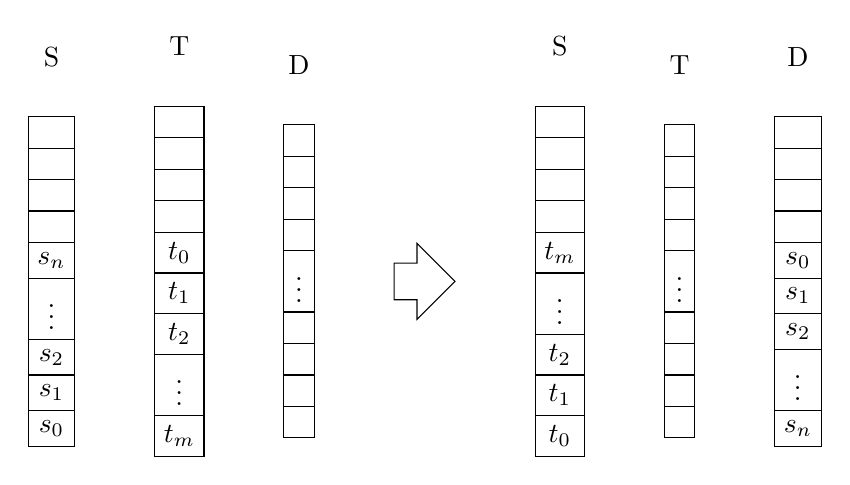
\begin{tikzpicture}[stack/.style={
                rectangle split, rectangle split parts=9, draw, anchor=center},
            myarrow/.style={single arrow, draw=none}]

            \node [stack] (s0)  {
            \nodepart{five}$s_n$
            \nodepart{six}$\vdots$\nodepart{seven}$s_2$\nodepart{eight}$s_1$
            \nodepart{nine}$s_0$};
            \node [stack,right=of s0] (t0) {
            \nodepart{nine}$t_m$
            \nodepart{eight}$\vdots$\nodepart{seven}$t_2$\nodepart{six}$t_1$
            \nodepart{five}$t_0$};
            \node [stack,right=of t0] (d0) {\nodepart{five}$\vdots$};
            \node [above=of s0,anchor=north,align=left] {S};
            \node [above=of t0,anchor=north,align=left] {T};
            \node [above=of d0,anchor=north,align=left] {D};

            \node [myarrow,draw,right=of d0] (a1) {\phantom{te}} ;

            \node [stack,right=of a1] (s1)  {
            \nodepart{five}$t_m$
            \nodepart{six}$\vdots$\nodepart{seven}$t_2$\nodepart{eight}$t_1$
            \nodepart{nine}$t_0$};
            \node [stack,right=of s1] (t1) {\nodepart{five}$\vdots$};
            \node [stack,right=of t1] (d1) {
            \nodepart{nine}$s_n$
            \nodepart{eight}$\vdots$\nodepart{seven}$s_2$\nodepart{six}$s_1$
            \nodepart{five}$s_0$};
            \node [above=of s1,anchor=north,align=left] {S};
            \node [above=of t1,anchor=north,align=left] {T};
            \node [above=of d1,anchor=north,align=left] {D};

        \end{tikzpicture}
        \caption{\alg{Pop} all elements from S and \alg{Push\_front} them to D. Then 
                 \alg{Pop} all elements from T to S.}
    \end{figure}

    \begin{figure}[h!]
        \centering
        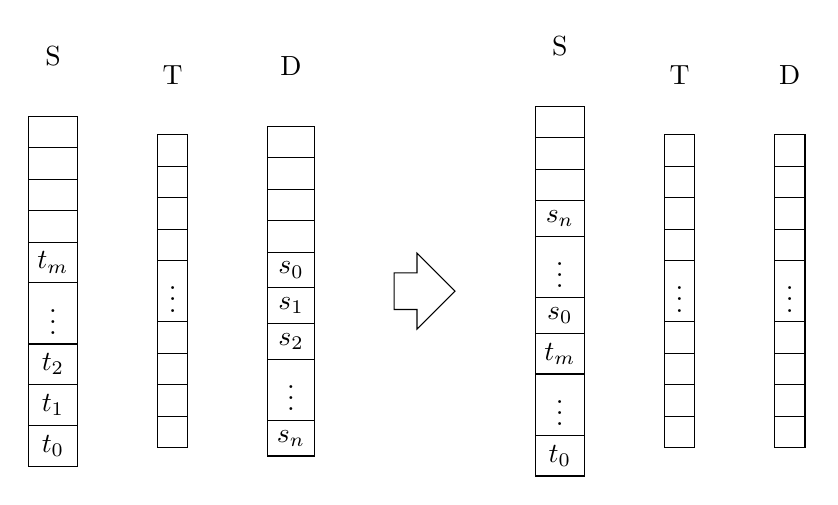
\begin{tikzpicture}[stack/.style={
                rectangle split, rectangle split parts=9, draw, anchor=center},
            myarrow/.style={single arrow, draw=none}]

            \node [stack] (s0)  {
            \nodepart{five}$t_m$
            \nodepart{six}$\vdots$\nodepart{seven}$t_2$\nodepart{eight}$t_1$
            \nodepart{nine}$t_0$};
            \node [stack,right=of s0] (t0) {\nodepart{five}$\vdots$};
            \node [stack,right=of t0] (d0) {
            \nodepart{nine}$s_n$
            \nodepart{eight}$\vdots$\nodepart{seven}$s_2$\nodepart{six}$s_1$
            \nodepart{five}$s_0$};

            \node [above=of s0,anchor=north,align=left] {S};
            \node [above=of t0,anchor=north,align=left] {T};
            \node [above=of d0,anchor=north,align=left] {D};

            \node [myarrow,draw,right=of d0] (a1) {\phantom{te}} ;

            \node [stack,right=of a1] (s1)  {
            \nodepart{four}$s_n$\nodepart{five}$\vdots$
            \nodepart{six}$s_0$\nodepart{seven}$t_m$
            \nodepart{eight}$\vdots$ \nodepart{nine}$t_0$};
            \node [stack,right=of s1] (t1) {\nodepart{five}$\vdots$};
            \node [stack,right=of t1] (d1) {\nodepart{five}$\vdots$};
            \node [above=of s1,anchor=north,align=left] {S};
            \node [above=of t1,anchor=north,align=left] {T};
            \node [above=of d1,anchor=north,align=left] {D};

        \end{tikzpicture}
        \caption{\alg{Pop\_front} all elements from D to S}
    \end{figure}


    \pagebreak

    \subqest{Use any pseudocode to write down an algorithm that uses two stacks 
    (with push, pop and isempty operations but no others) to simulate one deque
    (for push/pop front and push/pop back operations).
    What is the total running time after N operations?}

    Imagine we divide a deque into two stacks named $S_f$ and $S_b$. \alg{PushFront}, 
    \alg{PopFront} are processed in $S_f$ while \alg{PushBack}, \alg{PopBack} are
    processed in $S_b$. However, we need to transport elements from a stack to the other
    one if we want to \alg{Pop} elements from an empty stack. Note that both stacks
    are empty means the deque is empty.

    \begin{figure}[h!]
        \centering
        \begin{tikzpicture}
            \node[anchor=center] at (2,1) {$S_f$};
            \draw (0,0) -- (4,0) -- (4,2) -- (0,2) ;
            \node[anchor=center] at (7,1) {$S_b$};
            \draw (9,0) -- (5,0) -- (5,2) -- (9,2) ;
            \draw (0,3) -- (9,3) -- (9,4) -- (0,4) -- (0,3);
            \node[anchor=center] at (4.5,3.5) {$deque$};
        \end{tikzpicture}
        \caption{Use two stacks to simulate a deque}
    \end{figure}
    \begin{algorithm}[]
        \begin{algorithmic}[1]
            \Function{PopFront}{}
            \If{\emph{$S_f$ and $S_b$ aren't both empty}}
                \If{\emph{$S_f$ is empty}}
                    \State{\emph{pop all elements from $S_b$ to $S_f$}}
                \EndIf
                \State{\emph{pop from $S_f$}}
            \EndIf
            \EndFunction{}
        \end{algorithmic}
        \caption{PopFront of deque using two stacks}
    \end{algorithm}
    \begin{algorithm}[]
        \begin{algorithmic}[1]
            \Function{PopBack}{}
            \If{\emph{$S_f$ and $S_b$ aren't both empty}}
                \If{\emph{$S_b$ is empty}}
                    \State{\emph{pop all elements from $S_f$ to $S_b$}}
                \EndIf
                \State{\emph{pop from $S_b$}}
            \EndIf
            \EndFunction{}

        \end{algorithmic}
        \caption{PopBack of deque using two stacks}
    \end{algorithm}

    \pagebreak

    \begin{algorithm}[]
        \begin{algorithmic}[1]
            \Function{PushFront}{$e$}
                \State{\emph{push e into $S_f$}}
            \EndFunction{}
        \end{algorithmic}
        \caption{PushFront}
    \end{algorithm}
    \begin{algorithm}[]
        \begin{algorithmic}[1]
            \Function{PushBack}{$e$}
                \State{\emph{push e into $S_b$}}
            \EndFunction{}
        \end{algorithmic}
        \caption{PushBack}
    \end{algorithm}

    Suppose \alg{Pop}/\alg{Push} both take $t$ (Time Unit).
    There are some cases result in different running time.
    \begin{description}
    \item[Case 1:] all the operations are either \alg{PushBack} or \alg{PushFront} \\
        Since these two operations are just a \alg{Push} operation for a stack, the 
        time complexity is constant. After N operations, the total running time is 
        simply $Nt$.
    \item[Case 2:] operations contain \alg{PopBack} or \alg{PopFront}, but never make
        any stack empty \\
        Like Case 1, each opertation is either \alg{Push} or \alg{Pop} for a stack.
        Therefore, the total running time is also $Nt$.
    \item[Case 3:] operations contain \alg{PopBack} or \alg{PopFront}, and try to \alg{Pop}
        from an empty stack \\
        In this stituation, it would \alg{Pop} all elements from the other stack to its 
        first then \alg{Pop} the desired elements. Suppose this stituation happened $k$
        times, and there are $a_i$ elements in the other stack at the $i$th time.
        The total time is $N + \sum\limits_{i=1}^k a_i $.

    \end{description}


    \pagebreak
    
    \subqest{Do Exercise C-5.9 of the textbook, but with three stacks instead of two stacks and 
    one deque.}
    Suppose three stacks are big enough for all elements.

    \begin{figure}[h!]
        \centering
        \begin{tikzpicture}[stack/.style={
                rectangle split, rectangle split parts=9, draw, anchor=center},
            myarrow/.style={single arrow, draw=none}]

            \node [stack] (s0)  {
            \nodepart{five}$s_n$
            \nodepart{six}$\vdots$\nodepart{seven}$s_2$\nodepart{eight}$s_1$
            \nodepart{nine}$s_0$};
            \node [stack,right=of s0] (t0) {
            \nodepart{five}$t_m$
            \nodepart{six}$\vdots$\nodepart{seven}$t_2$\nodepart{eight}$t_1$
            \nodepart{nine}$t_0$};
            \node [stack,right=of t0] (e0) {\nodepart{five}$\vdots$};
            \node [above=of s0,anchor=north,align=left] {S};
            \node [above=of t0,anchor=north,align=left] {T};
            \node [above=of e0,anchor=north,align=left] {E};

            \node [myarrow,draw,right=of d0] (a1) {\phantom{te}} ;

            \node [stack,right=of a1] (s1) {\nodepart{five}$\vdots$};
            \node [stack,right=of s1] (t1) {\nodepart{five}$\vdots$};
            \node [stack,right=of t1] (e1) {
            \nodepart{nine}$s_n$\nodepart{eight}$\vdots$
            \nodepart{seven}$s_0$\nodepart{six}$t_m$
            \nodepart{five}$\vdots$ \nodepart{four}$t_0$};
            \node [above=of s1,anchor=north,align=left] {S};
            \node [above=of t1,anchor=north,align=left] {T};
            \node [above=of e1,anchor=north,align=left] {E};

        \end{tikzpicture}
        \caption{\alg{Pop} all elements from S to E and then \alg{Pop} all elements from T to E.}
    \end{figure}

    \begin{figure}[h!]
        \centering
        \begin{tikzpicture}[stack/.style={
                rectangle split, rectangle split parts=9, draw, anchor=center},
            myarrow/.style={single arrow, draw=none}]
            \node [stack] (s0) {\nodepart{five}$\vdots$};
            \node [stack,right=of s0] (t0) {\nodepart{five}$\vdots$};
            \node [stack,right=of t0] (e0) {
            \nodepart{nine}$s_n$\nodepart{eight}$\vdots$
            \nodepart{seven}$s_0$\nodepart{six}$t_m$
            \nodepart{five}$\vdots$ \nodepart{four}$t_0$};
            \node [above=of s0,anchor=north,align=left] {S};
            \node [above=of t0,anchor=north,align=left] {T};
            \node [above=of e0,anchor=north,align=left] {E};

            \node [myarrow,draw,right=of d0] (a1) {\phantom{te}} ;

            \node [stack,right=of a1] (s1)  {
            \nodepart{four}$s_n$\nodepart{five}$\vdots$
            \nodepart{six}$s_0$\nodepart{seven}$t_m$
            \nodepart{eight}$\vdots$ \nodepart{nine}$t_0$};
            \node [stack,right=of s1] (t1) {\nodepart{five}$\vdots$};
            \node [stack,right=of t1] (e1) {\nodepart{five}$\vdots$};
            \node [above=of s1,anchor=north,align=left] {S};
            \node [above=of t1,anchor=north,align=left] {T};
            \node [above=of e1,anchor=north,align=left] {E};

        \end{tikzpicture}
        \caption{\alg{Pop} all elements from E to S}
    \end{figure}

\end{homeworkProblem}


\pagebreak

\begin{homeworkProblem}{List, Iterator}
    \subqest{Do Exercise C-6.7 of the textbook.}
    Like textbook, we view the computer as a coin-operated appliance, which requires
    the payment of one \textbf{cyber-dollar} for a constant amount of computing time.
    Suppose it costs 6 cyber-dollars to push one element to a non-full array. In fact,
    only one cyber-dollars is used to insert an element, and the other five are just
    stored in the place. Consider a case that an array just extended its size from 
    $N$ to $N + \lceil \frac{N}{4} \rceil$. After pushing $\lceil \frac{N}{4} \rceil$ elements, 
    the array is full again. Note that we stored at least 
    $5 \times \lceil \frac{N}{4}\rceil$ cyber-dollars at this moment. Next time before
    we push a new element, we would have to copy $N + \lceil \frac{N}{4} \rceil$
    elements from old array to a new array. And we know that
    \[
        \begin{split}
            5 \times \lceil \frac{N}{4}\rceil &= 4 \times \lceil \frac{N}{4}\rceil + \lceil \frac{N}{4}\rceil \\
            &\geq N + \lceil \frac{N}{4}\rceil
        \end{split}
    \]
    It means we can use the cyber-dollars we stored before to copy elements without 
    running out of the money. That is, the real average cost of pushing a element 
    to an array is less than 6 cyber-dollars. Therefore, it totally costs less than $6n$
    cyber-dollars after a sequence of $n$ push operations. This implies it still run in
    $O(n)$ in this case.

    

    \subqest{Do Exercise C-6.13 of the textbook by Googling the \textit{Knuth Shuffle}.}

    \begin{algorithm}[]
        \begin{algorithmic}[1]
            \Function{Knuth-Shuffle}{$V, LengthOfV$}
            \For{$i \gets 0$ to $LengthOfV -1$}
                \State{$r \gets$ \Call{randomIntger}{$i+1$}}
                \State{$Exchange~\alg{V[i]}~and~\alg{V[r]}$}
            \EndFor
            \EndFunction{}
        \end{algorithmic}
        \caption{Knuth-Shuffle}
    \end{algorithm}

    Knuth Shuffle guarantees that every possible ordering is equally likely. The running time
    of this function is $O(n)$, $n$ is the number of cards.


\end{homeworkProblem}


\pagebreak

\begin{homeworkProblem}{Calculators}
    \subqest{Three cases for testing integer calculator}

    \begin{lstlisting}[breaklines=true]
    Input:

    123+2*3*(5-3+48/2) + 34
    -~((1024 >> (23 % 3)) + !0)
    ((3 && +1 || 1) ^ 12 << 1 ) & 16 | 2
    ---
    Output:

    --- postfix expression transforming ---
    encounter 123: push to output
            current output: 123
    encounter +: push to the stack directly
            current output: 123
            current stack:  +
    encounter 2: push to output
            current output: 123 2
            current stack:  +
    encounter *: push to the stack directly
            current output: 123 2
            current stack:  + *
    encounter 3: push to output
            current output: 123 2 3
            current stack:  + *
    encounter *: stack.top() has greater or the same precdence, after pop something out to output, then push to the stack
            current output: 123 2 3 *
            current stack:  + *
    encounter (: push to the stack directly
            current output: 123 2 3 *
            current stack:  + * (
    encounter 5: push to output
            current output: 123 2 3 * 5
            current stack:  + * (
    encounter -: push to the stack directly
            current output: 123 2 3 * 5
            current stack:  + * ( -
    encounter 3: push to output
            current output: 123 2 3 * 5 3
            current stack:  + * ( -
    encounter +: stack.top() has greater or the same precdence, after pop something out to output, then push to the stack
            current output: 123 2 3 * 5 3 -
            current stack:  + * ( +
    encounter 48: push to output
            current output: 123 2 3 * 5 3 - 48
            current stack:  + * ( +
    encounter /: push to the stack directly
            current output: 123 2 3 * 5 3 - 48
            current stack:  + * ( + /
    encounter 2: push to output
            current output: 123 2 3 * 5 3 - 48 2
            current stack:  + * ( + /
    encounter ): flush the stack to output until meeting '('
            current output: 123 2 3 * 5 3 - 48 2 / +
            current stack:  + *
    encounter +: stack.top() has greater or the same precdence, after pop something out to output, then push to the stack
            current output: 123 2 3 * 5 3 - 48 2 / + * +
            current stack:  +
    encounter 34: push to output
            current output: 123 2 3 * 5 3 - 48 2 / + * + 34
            current stack:  +
    encounter NOTHING: flush the stack to output
            current output: 123 2 3 * 5 3 - 48 2 / + * + 34 +
    --- postfix expression transforming complete :) ---
    Postfix Exp: 123 2 3 * 5 3 - 48 2 / + * + 34 +
    RESULT: 313
    --- postfix expression transforming ---
    encounter U-: push to the stack directly
            current output:
            current stack:  -
    encounter ~: push to the stack directly
            current output:
            current stack:  - ~
    encounter (: push to the stack directly
            current output:
            current stack:  - ~ (
    encounter (: push to the stack directly
            current output:
            current stack:  - ~ ( (
    encounter 1024: push to output
            current output: 1024
            current stack:  - ~ ( (
    encounter >>: push to the stack directly
            current output: 1024
            current stack:  - ~ ( ( >>
    encounter (: push to the stack directly
            current output: 1024
            current stack:  - ~ ( ( >> (
    encounter 23: push to output
            current output: 1024 23
            current stack:  - ~ ( ( >> (
    encounter %: push to the stack directly
            current output: 1024 23
            current stack:  - ~ ( ( >> ( %
    encounter 3: push to output
            current output: 1024 23 3
            current stack:  - ~ ( ( >> ( %
    encounter ): flush the stack to output until meeting '('
            current output: 1024 23 3 %
            current stack:  - ~ ( ( >>
    encounter ): flush the stack to output until meeting '('
            current output: 1024 23 3 % >>
            current stack:  - ~ (
    encounter +: push to the stack directly
            current output: 1024 23 3 % >>
            current stack:  - ~ ( +
    encounter !: push to the stack directly
            current output: 1024 23 3 % >>
            current stack:  - ~ ( + !
    encounter 0: push to output
            current output: 1024 23 3 % >> 0
            current stack:  - ~ ( + !
    encounter ): flush the stack to output until meeting '('
            current output: 1024 23 3 % >> 0 ! +
            current stack:  - ~
    encounter NOTHING: flush the stack to output
            current output: 1024 23 3 % >> 0 ! + ~ -
    --- postfix expression transforming complete :) ---
    Postfix Exp: 1024 23 3 % >> 0 ! + ~ -
    RESULT: 258
    --- postfix expression transforming ---
    encounter (: push to the stack directly
            current output:
            current stack:  (
    encounter (: push to the stack directly
            current output:
            current stack:  ( (
    encounter 3: push to output
            current output: 3
            current stack:  ( (
    encounter &&: push to the stack directly
            current output: 3
            current stack:  ( ( &&
    encounter U+: push to the stack directly
            current output: 3
            current stack:  ( ( && +
    encounter 1: push to output
            current output: 3 1
            current stack:  ( ( && +
    encounter ||: stack.top() has greater or the same precdence, after pop something out to output, then push to the stack
            current output: 3 1 + &&
            current stack:  ( ( ||
    encounter 1: push to output
            current output: 3 1 + && 1
            current stack:  ( ( ||
    encounter ): flush the stack to output until meeting '('
            current output: 3 1 + && 1 ||
            current stack:  (
    encounter ^: push to the stack directly
            current output: 3 1 + && 1 ||
            current stack:  ( ^
    encounter 12: push to output
            current output: 3 1 + && 1 || 12
            current stack:  ( ^
    encounter <<: push to the stack directly
            current output: 3 1 + && 1 || 12
            current stack:  ( ^ <<
    encounter 1: push to output
            current output: 3 1 + && 1 || 12 1
            current stack:  ( ^ <<
    encounter ): flush the stack to output until meeting '('
            current output: 3 1 + && 1 || 12 1 << ^
    encounter &: push to the stack directly
            current output: 3 1 + && 1 || 12 1 << ^
            current stack:  &
    encounter 16: push to output
            current output: 3 1 + && 1 || 12 1 << ^ 16
            current stack:  &
    encounter |: stack.top() has greater or the same precdence, after pop something out to output, then push to the stack
            current output: 3 1 + && 1 || 12 1 << ^ 16 &
            current stack:  |
    encounter 2: push to output
            current output: 3 1 + && 1 || 12 1 << ^ 16 & 2
            current stack:  |
    encounter NOTHING: flush the stack to output
            current output: 3 1 + && 1 || 12 1 << ^ 16 & 2 |
    --- postfix expression transforming complete :) ---
    Postfix Exp: 3 1 + && 1 || 12 1 << ^ 16 & 2 |
    RESULT: 18
    \end{lstlisting}

    \subqest{Three cases for testing scientific calculator}

    \begin{lstlisting}[breaklines=true]
    Input:

    - pow( (2.3 + 3) *2 , exp( log(2) ) )
    sqrt(1/16) + fabs(sin(3 / 2 * 3.1415926)) + +cos(3.1415926)
    0.00 + 1.2
    ---
    Output:

    --- postfix expression transforming ---
    encounter U-: push to the stack directly
            current output:
            current stack:  -
    encounter pow: push to the stack directly
            current output:
            current stack:  - pow
    encounter (: push to the stack directly
            current output:
            current stack:  - pow (
    encounter (: push to the stack directly
            current output:
            current stack:  - pow ( (
    encounter 2.3: push to output
            current output: 2.300000
            current stack:  - pow ( (
    encounter +: push to the stack directly
            current output: 2.300000
            current stack:  - pow ( ( +
    encounter 3: push to output
            current output: 2.300000 3.000000
            current stack:  - pow ( ( +
    encounter ): flush the stack to output until meeting '(' 
            current output: 2.300000 3.000000 +
            current stack:  - pow (
    encounter *: push to the stack directly
            current output: 2.300000 3.000000 +
            current stack:  - pow ( *
    encounter 2: push to output
            current output: 2.300000 3.000000 + 2.000000
            current stack:  - pow ( *
    encounter exp: push to the stack directly
            current output: 2.300000 3.000000 + 2.000000
            current stack:  - pow ( * exp
    encounter (: push to the stack directly
            current output: 2.300000 3.000000 + 2.000000
            current stack:  - pow ( * exp (
    encounter log: push to the stack directly
            current output: 2.300000 3.000000 + 2.000000
            current stack:  - pow ( * exp ( log
    encounter (: push to the stack directly
            current output: 2.300000 3.000000 + 2.000000
            current stack:  - pow ( * exp ( log (
    encounter 2: push to output
            current output: 2.300000 3.000000 + 2.000000 2.000000
            current stack:  - pow ( * exp ( log (
    encounter ): flush the stack to output until meeting '(' and pop function 'log' to output
            current output: 2.300000 3.000000 + 2.000000 2.000000 log
            current stack:  - pow ( * exp (
    encounter ): flush the stack to output until meeting '(' and pop function 'exp' to output
            current output: 2.300000 3.000000 + 2.000000 2.000000 log exp
            current stack:  - pow ( *
    encounter ): flush the stack to output until meeting '(' and pop function 'pow' to output
            current output: 2.300000 3.000000 + 2.000000 2.000000 log exp * pow
            current stack:  -
    encounter NOTHING: flush the stack to output
            current output: 2.300000 3.000000 + 2.000000 2.000000 log exp * pow -
    --- postfix expression transforming complete :) ---
    Postfix Exp: 2.300000 3.000000 + 2.000000 2.000000 log exp * pow -
    RESULT: -789.048100
    --- postfix expression transforming ---
    encounter sqrt: push to the stack directly
            current output:
            current stack:  sqrt
    encounter (: push to the stack directly
            current output:
            current stack:  sqrt (
    encounter 1: push to output
            current output: 1.000000
            current stack:  sqrt (
    encounter /: push to the stack directly
            current output: 1.000000
            current stack:  sqrt ( /
    encounter 16: push to output
            current output: 1.000000 16.000000
            current stack:  sqrt ( /
    encounter ): flush the stack to output until meeting '(' and pop function 'sqrt' to output
            current output: 1.000000 16.000000 / sqrt
    encounter +: push to the stack directly
            current output: 1.000000 16.000000 / sqrt
            current stack:  +
    encounter fabs: push to the stack directly
            current output: 1.000000 16.000000 / sqrt
            current stack:  + fabs
    encounter (: push to the stack directly
            current output: 1.000000 16.000000 / sqrt
            current stack:  + fabs (
    encounter sin: push to the stack directly
            current output: 1.000000 16.000000 / sqrt
            current stack:  + fabs ( sin
    encounter (: push to the stack directly
            current output: 1.000000 16.000000 / sqrt
            current stack:  + fabs ( sin (
    encounter 3: push to output
            current output: 1.000000 16.000000 / sqrt 3.000000
            current stack:  + fabs ( sin (
    encounter /: push to the stack directly
            current output: 1.000000 16.000000 / sqrt 3.000000
            current stack:  + fabs ( sin ( /
    encounter 2: push to output
            current output: 1.000000 16.000000 / sqrt 3.000000 2.000000
            current stack:  + fabs ( sin ( /
    encounter *: stack.top() has greater or the same precdence, after pop something out to output, then push to the stack
            current output: 1.000000 16.000000 / sqrt 3.000000 2.000000 /
            current stack:  + fabs ( sin ( *
    encounter 3.1415926: push to output
            current output: 1.000000 16.000000 / sqrt 3.000000 2.000000 / 3.141593
            current stack:  + fabs ( sin ( *
    encounter ): flush the stack to output until meeting '(' and pop function 'sin' to output
            current output: 1.000000 16.000000 / sqrt 3.000000 2.000000 / 3.141593 * sin
            current stack:  + fabs (
    encounter ): flush the stack to output until meeting '(' and pop function 'fabs' to output
            current output: 1.000000 16.000000 / sqrt 3.000000 2.000000 / 3.141593 * sin fabs
            current stack:  +
    encounter +: stack.top() has greater or the same precdence, after pop something out to output, then push to the stack
            current output: 1.000000 16.000000 / sqrt 3.000000 2.000000 / 3.141593 * sin fabs +
            current stack:  +
    encounter U+: push to the stack directly
            current output: 1.000000 16.000000 / sqrt 3.000000 2.000000 / 3.141593 * sin fabs +
            current stack:  + +
    encounter cos: push to the stack directly
            current output: 1.000000 16.000000 / sqrt 3.000000 2.000000 / 3.141593 * sin fabs +
            current stack:  + + cos
    encounter (: push to the stack directly
            current output: 1.000000 16.000000 / sqrt 3.000000 2.000000 / 3.141593 * sin fabs +
            current stack:  + + cos (
    encounter 3.1415926: push to output
            current output: 1.000000 16.000000 / sqrt 3.000000 2.000000 / 3.141593 * sin fabs + 3.141593
            current stack:  + + cos (
    encounter ): flush the stack to output until meeting '(' and pop function 'cos' to output
            current output: 1.000000 16.000000 / sqrt 3.000000 2.000000 / 3.141593 * sin fabs + 3.141593 cos
            current stack:  + +
    encounter NOTHING: flush the stack to output
            current output: 1.000000 16.000000 / sqrt 3.000000 2.000000 / 3.141593 * sin fabs + 3.141593 cos + +
    --- postfix expression transforming complete :) ---
    Postfix Exp: 1.000000 16.000000 / sqrt 3.000000 2.000000 / 3.141593 * sin fabs + 3.141593 cos + +
    RESULT: 0.250000
    --- postfix expression transforming ---
    encounter 0.00: push to output
            current output: 0.000000
    encounter +: push to the stack directly
            current output: 0.000000
            current stack:  +
    encounter 1.2: push to output
            current output: 0.000000 1.200000
            current stack:  +
    encounter NOTHING: flush the stack to output
            current output: 0.000000 1.200000 +
    --- postfix expression transforming complete :) ---
    Postfix Exp: 0.000000 1.200000 +
    RESULT: 1.200000
    \end{lstlisting}

\end{homeworkProblem}

\end{document}
